\documentclass{standalone}
\usepackage{tikz}
\usepackage{pgfplots}
\usepgfplotslibrary{colorbrewer}
\usepackage{nono}
\usepackage{siunitx}
\pgfplotsset{
  colormap={custom}{rgb255(0cm)=(255,0,0); rgb255(1cm)=(255,255,255);}
}
\begin{document}
%\usepgfplotslibrary{colormaps} 
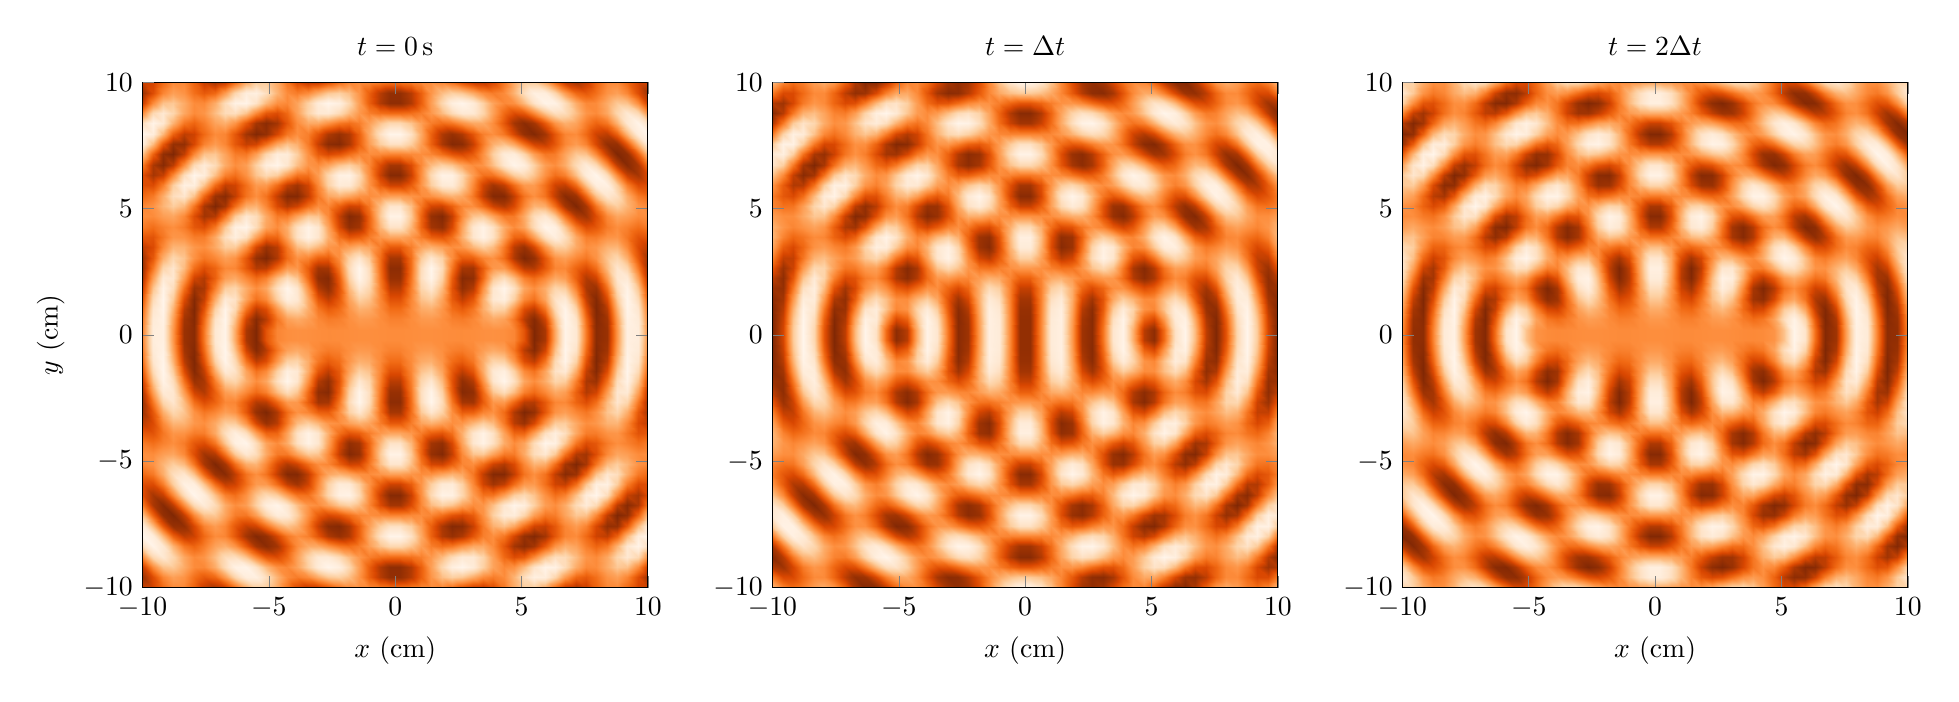
\begin{tikzpicture} 
% Define custom colormap
\begin{axis}[view={0}{90},
		xlabel=$x$ (cm),
		ylabel=$y$ (cm),
    title = {$t=\SI{0}{s}$},
		axis equal,
		width=8cm,
		height=8cm,
    xmin=-10,xmax=10,ymin=-10, ymax=10,
    colormap/Oranges-9]
		\addplot3[surf, shader=interp,domain=-10:10, samples=50] {cos(-90+144*sqrt(((x+5)^2 + y^2)))+cos(-90+144*sqrt(((x-5)^2 + y^2)))};
\end{axis}
\begin{scope}[xshift=8cm]
\begin{axis}[view={0}{90},
		xlabel=$x$ (cm),
    title = {$t=\Delta t$},
		axis equal,
		width=8cm,
		height=8cm,
    ylabel={},
    xmin=-10,xmax=10,ymin=-10, ymax=10,
    colormap/Oranges-9]
		\addplot3[surf, shader=interp,domain=-10:10, samples=50] {cos(144*sqrt(((x+5)^2 + y^2)))+cos(144*sqrt(((x-5)^2 + y^2)))};
\end{axis}
\end{scope}
\begin{scope}[xshift=16cm]
\begin{axis}[view={0}{90},
		xlabel=$x$ (cm),
    title = {$t=2\Delta t$},
		axis equal,
		width=8cm,
		height=8cm,
    xmin=-10,xmax=10,ymin=-10, ymax=10,
    colormap/Oranges-9]
		\addplot3[surf, shader=interp,domain=-10:10, samples=50] {cos(90+144*sqrt(((x+5)^2 + y^2)))+cos(90+144*sqrt(((x-5)^2 + y^2)))};
\end{axis}
\end{scope}
\end{tikzpicture}
\end{document}
